%\documentclass[dvipdfmx,autodetect-engine]{jreport}
\documentclass[xelatex,ja=standard]{bxjsarticle}
\usepackage[dvipdfmx]{graphicx}
\usepackage[utf8]{inputenc}
\usepackage{listings}
\lstset{
 	language = Python,
	breaklines = true,
	basicstyle=\ttfamily\scriptsize,
	commentstyle={\textmc},
	classoffset=1,
	keywordstyle=\bfseries,
	showstringspaces=false,
	frame=tblr,
	numbers=left,
	stepnumber=1,
	numberstyle=\tiny,
	tabsize=2
}
%\usepackage[dvipdfmx]{graphicx}
%\usepackage[version=4]{mhchem}
\begin{document}

%overleaf使用の場合、メニューからコンパイラとしてXeLaTeXを選択してください。

\title{レポートタイトル}
\author{学科 学籍番号 氏名}
\date{2023年??月??日}
\maketitle
\section{はじめに}

\begin{figure}[htbp]
    \centering
    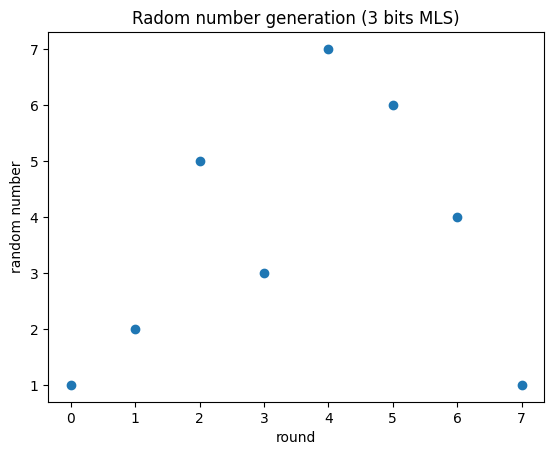
\includegraphics[scale=0.5]
{sample.png}
    \caption{図の貼り方}
    \label{fig:sample_figure}
\end{figure}

\section{実験1-5}

\subsection{目的}

これからランダムウォーク実験を行うにあたって、ランダムな数を生成することが必要であるが、パソコンはランダムな数を生成できない。そこでコンピューター上では数式を用いて擬似乱数列ー乱数のように思えるが、初期状態が決定すれば未来の数列が決定してしまうので真にランダムではない数列ーを生成するのだが、このときC言語における srand(time(NULL)) や、pythonにおける rand() のようないわゆる組み込み関数を用いずに擬似乱数列を生成するのが今回の実験の目的である。

\subsection{理論}

擬似乱数列の生成を行う。このとき LFSR 法を用いた。LFSR とは次の数を直前の数に基づきシフト演算を使って漸化式的に決定した数列(次の数が直前の数の線形写像になっているシフトレジスタ)のことで、このとき直前の数から次の数を求める漸化式をうまく設定することで、全ビットが0という状態以外のすべての取る整数列を作ることができることが分かっており、これを最長LFSR と呼ぶ。今回はこの最長LSFR を作ることで擬似乱数列を生成した。

ここで、最長LSFR を生成できる漸化式を次に示す。このとき、下に示す漸化式は2進数である
\[
a_{n+1}  = b_{n+1} + c_{n+1} \& 1
\]

但し

\[
b_{n+1} = ( a_{n} << 1 ) \& (10^{bit} - 1)
\]

(しつこいようだが、10はいわゆる2進数の10であり、つまり10進数における2である)

\[
c_{n+1} = \sum_{i} (a_n >> k_i)
\]

このとき、$ c_{n+1} $ を以下のように設定することで、最長LFSR を計算することができる:

\begin{figure}[htbp]
    \centering
    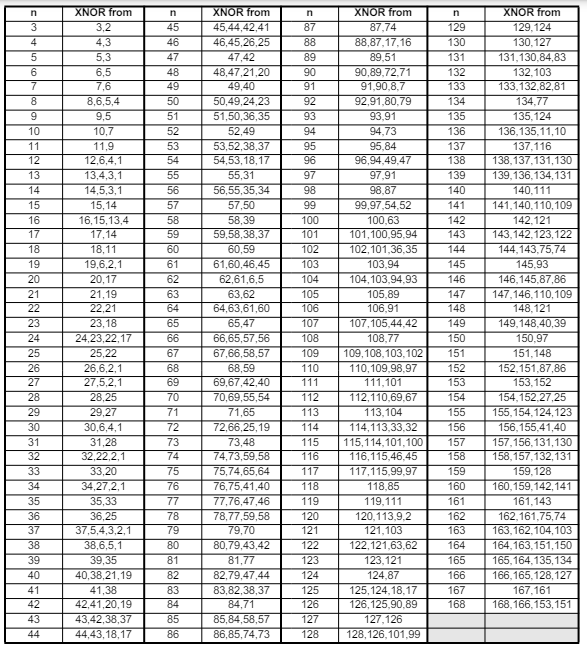
\includegraphics[scale=1]
{1.png}
    \label{fig:1}
\end{figure}

但し、漸化式中の $bit$、$k_i$ は、表にある表現を用いて
\[
bit = n
\]
\[
k_i = {XNOR from}
\]
と表せる


\subsection{実験方法}

実験に用いたpythonプログラムを次に示す
\lstinputlisting[caption = キャプション2 ,label = program2]{1.py}

\subsection{実験結果}

このプログラムを15bitで実行した結果を次に示す

\begin{figure}[htbp]
    \centering
    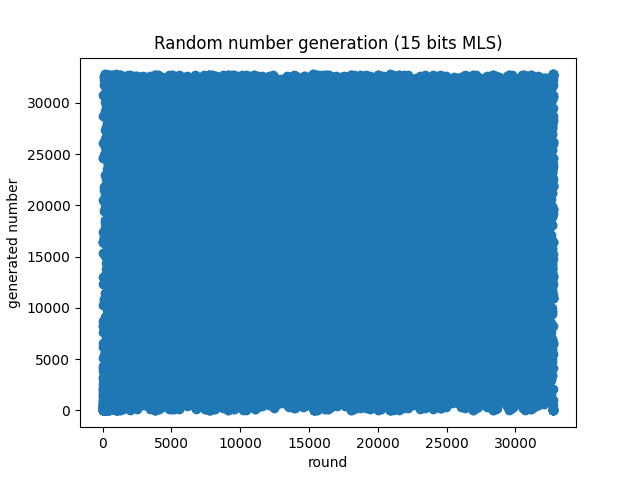
\includegraphics[scale=0.7]
{2.png}
    \label{fig:1}
\end{figure}

\begin{figure}[htbp]
    \centering
    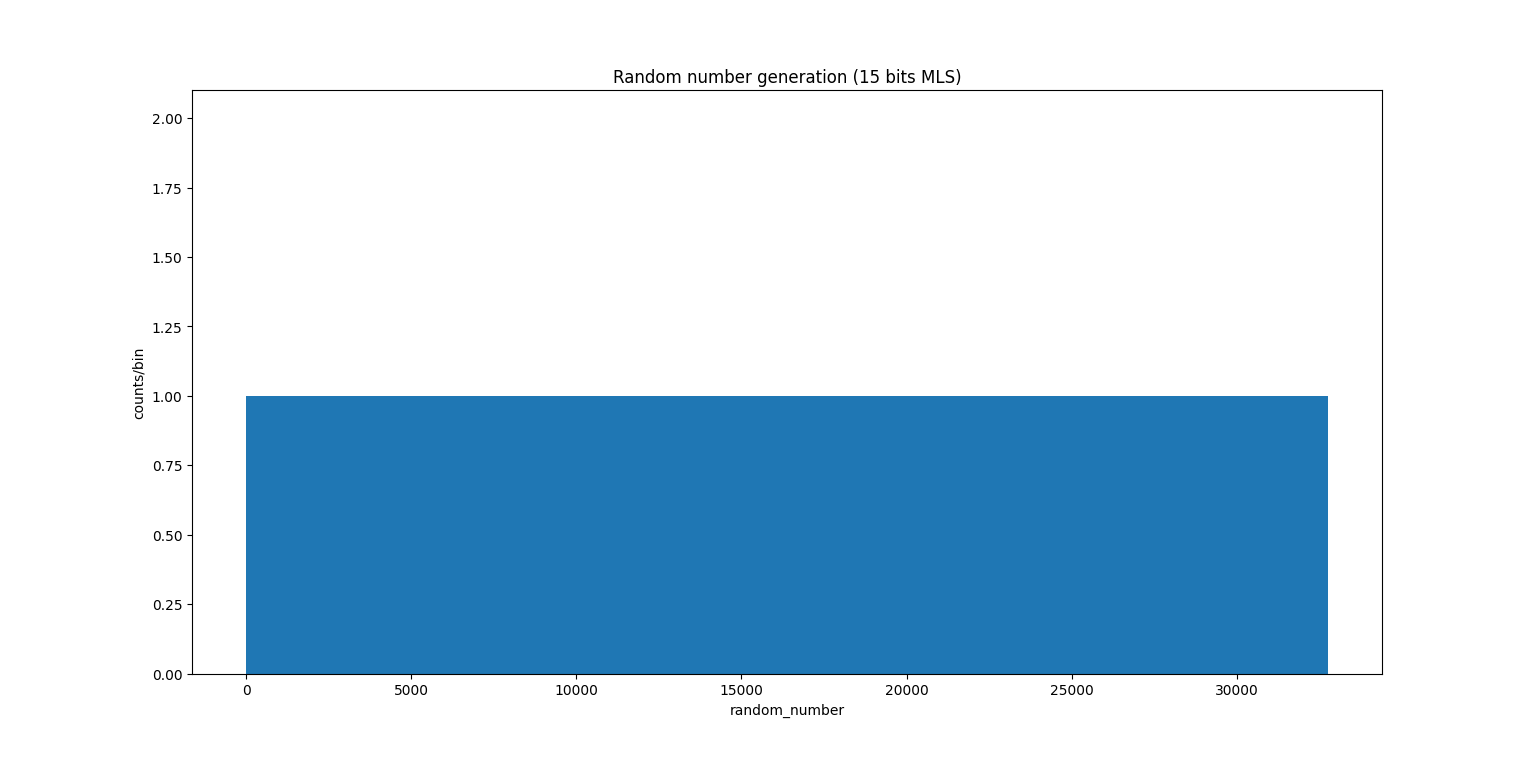
\includegraphics[scale=0.3]
{3.png}
    \label{fig:1}
\end{figure}

\begin{figure}[htbp]
    \centering
    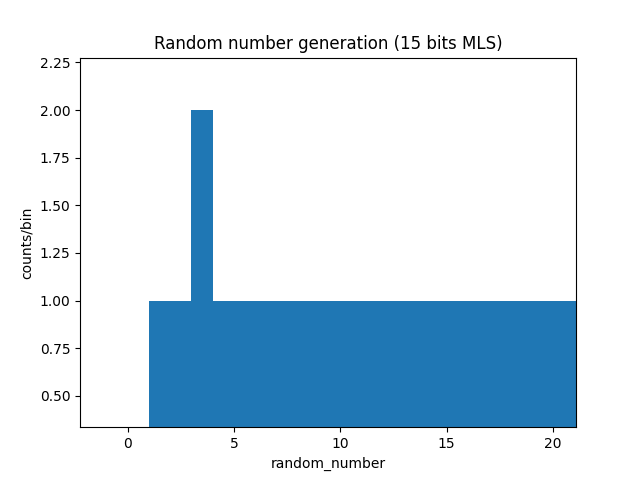
\includegraphics[scale=0.7]
{3-2.png}
    \label{fig:1}
\end{figure}


ここに示したヒストグラムのように、初期値である3 (ソースコード 1.py の54行目で指定した) を除いた全ての数が1から $2^{15}$ まで1回ずつのみ現れ、3のみ2回現れている。


\section{実験2}

\subsection{目的}
$Z^d ( \in j = (j_1,j_2 ... , j_d)) $ と表現されるd次元格子において、毎回2d個の隣接点から1点を等確率で選んで進んでいく運動をd次元単純ランダムウォークと呼ぶ。これはブラウン運動などと共に、統計力学・量子力学・数理ファイナンスのようなランダムな運動を数学的に記述するモデルのなかで、もっとも基本的なものの一つとして知られている。今回はそのなかでもっとも基礎的な1次元単純ランダムウォークを実行し、粒子の動きを調べることで、確率過程モデルの基礎を確認する。
\subsection{理論}
t回目の試行における粒子の座標を $x_t$ とおくと、
\[ 
P(x_{t+1} - x_{t} = 1) = 1/2
\]
\[
P(x_{t+1} - x_{t} = -1) = 1/2
\]
を満たすとする(単純ランダムウォーク)
\subsection{実験方法}
\subsubsection{実験2-4}
実験に用いたPythonプログラムを次に示す

\lstinputlisting[caption = キャプション2 ,label = program2]{2-1.py}

\subsubsection{実験2-5}
実験に用いたPythonプログラムを次に示す

\lstinputlisting[caption = キャプション2 ,label = program2]{2-2.py}

\subsection{実験結果}

\subsubsection{実験2-4}
実験の結果を次に示す
\begin{figure}[htbp]
    \centering
    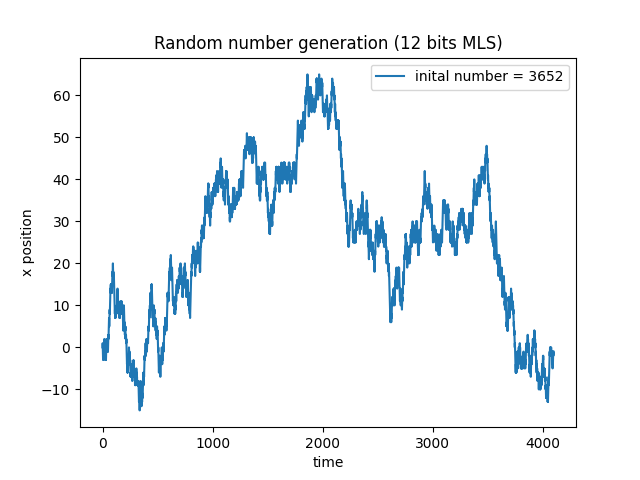
\includegraphics[scale=0.7]
{4.png}
    \label{fig:1}
\end{figure}

\subsubsection{実験2-5}
実験の結果を次に示す
\begin{figure}[htbp]
    \centering
    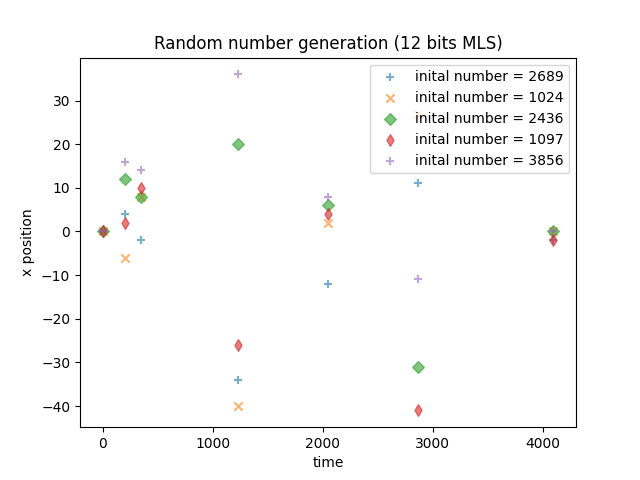
\includegraphics[scale=0.7]
{5.png}
    \label{fig:1}
\end{figure}

\section{実験3}

\subsection{目的}

\subsection{理論}

\subsection{実験方法}

\subsubsection{実験3-1}
実験に用いたPythonプログラムを次に示す
\lstinputlisting[caption = キャプション2 ,label = program2]{3-1.py}

\subsubsection{実験3-2,3-3}
実験に用いたPythonプログラムを次に示す
\lstinputlisting[caption = キャプション2 ,label = program2]{3-2.py}

\subsection{実験結果}

\subsubsection{実験3-1}
実験の結果を次に示す
\begin{figure}[htbp]
    \centering
    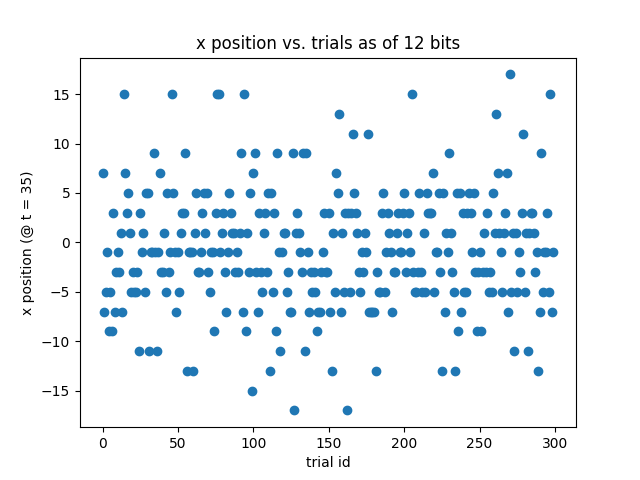
\includegraphics[scale=0.7]
{6.png}
    \label{fig:1}
\end{figure}

\subsubsection{実験3-2,3-3}
実験の結果を次に示す
\begin{figure}[htbp]
    \centering
    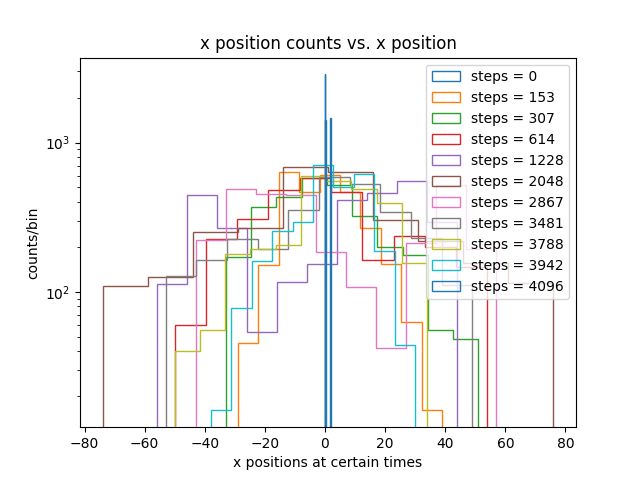
\includegraphics[scale=0.7]
{7.png}
    \label{fig:1}
\end{figure}

\begin{figure}[htbp]
    \centering
    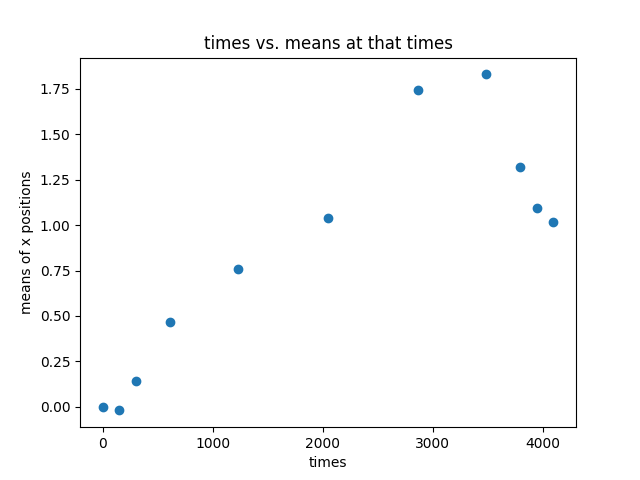
\includegraphics[scale=0.7]
{7-2.png}
    \label{fig:1}
\end{figure}

\begin{figure}[htbp]
    \centering
    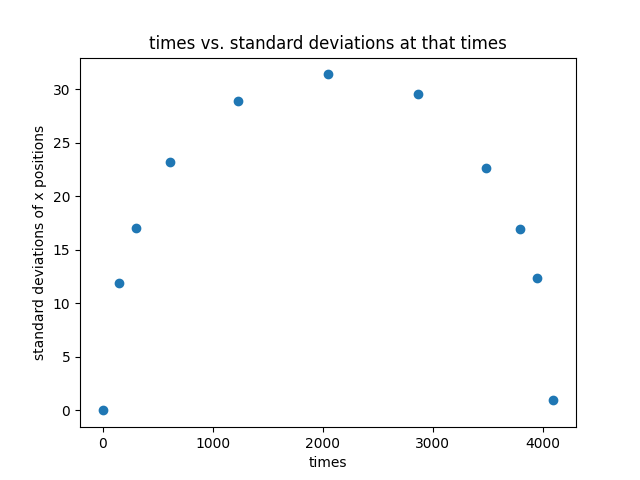
\includegraphics[scale=0.7]
{7-3.png}
    \label{fig:1}
\end{figure}


\end{document}
